\documentclass[14pt]{matmex-diploma}

\usepackage[]{algorithm2e}

\newenvironment{rualgorithm}[1][htb]
  {\renewcommand{\algorithmcfname}{Алгоритм}
   \begin{algorithm}[#1]
  }{\end{algorithm}}

\begin{document}
\filltitle{ru}{
    chair              = {Кафедра Системного Программирования},
    title              = {Оптимизация алгоритма лексического анализа динамически формируемого кода},
    type               = {coursework},
    position           = {студента},
    group              = 371,
    author             = {Байгельдин Александр Юрьевич},
    supervisorPosition = {ст.пр., магистр ИТ},
    supervisor         = {Григорьев С.\,В.},
    university         = {Санкт-Петербургский Государственный Университет},
}
\filltitle{en}{
    chair              = {Chair of Software Engineering},
    title              = {Optimization of lexical analysys of dynamically generated string expressions},
    author             = {Alexander Baygeldin},
    supervisorPosition = {senior lecturer, master of IT},
    supervisor         = {Semyon Grigoriyev},
    type               = {coursework},
}
\maketitle
\tableofcontents

\section*{Введение}
Динамически формируемый код — это код, который может быть получен и использован внутри другого кода при помощи строковых операций, таких как конкатенация, циклы, замена подстроки. Яркий пример такого кода — запросы SQL, которые составляются динамически в языках более общего назначения (C\#, PHP и др.). На рис.~\ref{пример_кода_1} представлен пример кода, составленного с помощью условного выражения и конкатенаций. 

\begin{figure}[h]
\centering
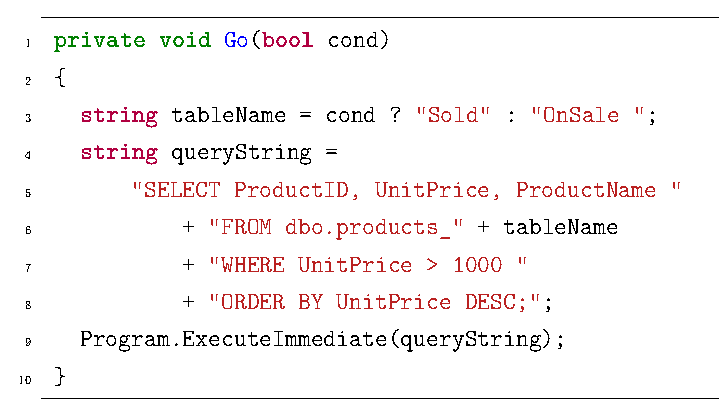
\includegraphics{pictures/intro_code.pdf}
\caption{Пример динамически формируемого кода}
\label{пример_кода_1}
\end{figure}

Однако в третьей строке примера при формировании имени таблицы был пропущен пробел, и эта ошибка будет выявлена только во время выполнения программы. Таким образом, при разработке и реинжиниринге систем, использующих динамически формируемый код, можно было бы избежать множество проблем, если бы в IDE существовала поддержка статического анализа подобного кода \cite{string_embedded}. Лексический анализ является важным шагом такого статического анализа.

Задача лексического анализа — выделение лексем во входном потоке и сохранение привязки, т.е. позиции в тексте, к исходному коду. Часто при лексическом анализе используются инструменты для генерации лексических анализаторов по спецификации языка. Лексический анализатор переводит поток символов в поток лексем и может быть представлен в виде конечного преобразователя. \textbf{Конечный преобразователь} (Finite State Transducer) — это математическая модель устройства, похожая на конечный автомат, с тем лишь дополнением, что каждому переходу сопоставляется дополнительное значение, которое выводится в выходной поток. На рис.~\ref{пример_лексического_анализатора} продемонстрирован пример лексического анализатора языка арифметических выражений (ради простоты, единственной операций является операция сложения), представленного в виде конечного преобразователя.

\begin{figure}[h]
\centering
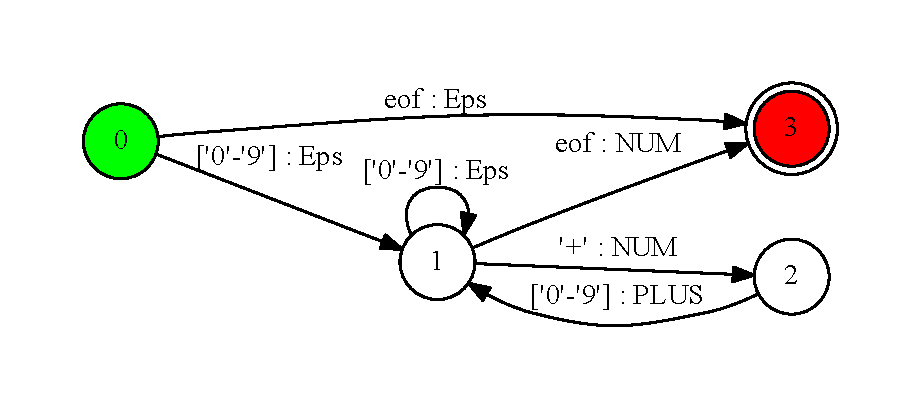
\includegraphics{pictures/lexer.pdf}
\caption{Пример лексического анализатора, представленного в виде FST}
\label{пример_лексического_анализатора}
\end{figure}

Однако большинство инструментов для генерации лексических анализаторов могут работать лишь с линейным входом, что делает невозможным их непосредственное применение в нашем случае, т.к. поток символов формируется динамически. Одно из возможных решений \cite{polubelova} заключается в построении регулярной аппроксимации множества значений динамически формируемого выражения и последующем применении операции композиции \cite{handbook_automata} к двум конечным преобразователям: один их них построен по регулярной аппроксимации преобразованием автомата над строками в автомат над символами, а второй является классическим лексическим анализатором для языка, на котором написан динамически формируемый код. На рис.~\ref{пример_регулярной_аппроксимации} изображен пример регулярной аппроксимации динамически формируемого кода, представленной в виде конечного автомата, построенного на основе кода на рис.~\ref{пример_кода_2}. 

\begin{figure}[h]
\centering
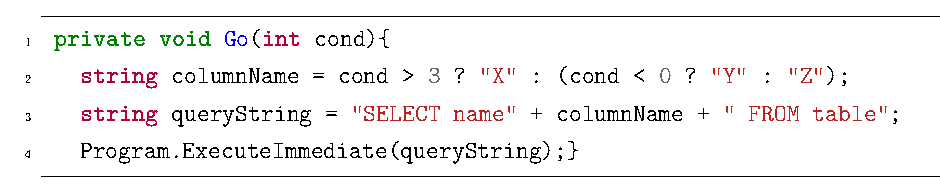
\includegraphics{pictures/approx_code.pdf}
\caption{Пример динамически формируемого кода}
\label{пример_кода_2}
\end{figure}

\begin{figure}[h]
\centering
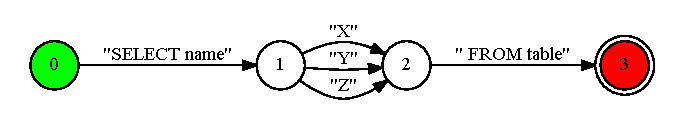
\includegraphics{pictures/approx_fsa.pdf}
\caption{Пример регулярной аппроксимации динамически формируемого кода}
\label{пример_регулярной_аппроксимации}
\end{figure}

Результатом операции композиции конечных преобразователей является конечный преобразователь, который обладает тем свойством, что результат его работы совпадает с результатом последовательного применения участников композиции на том же входе. В нашем случае, первый конечный преобразователь переводит поток символов с их привязкой к исходному коду в поток символов, а второй (лексический анализатор) переводит поток символов в поток лексем. Таким образом, результирующий конечный преобразователь переводит поток символов с их привязкой к исходному коду в поток лексем, что и является целью лексического анализа. Результатом применения операции композиции к конечному преобразователю на рис.~\ref{участник_композиции} и лексическому анализатору на рис. 2 является конечный преобразователь изображенный на рис.~\ref{результат_композиции}.

\begin{figure}[h]
\centering
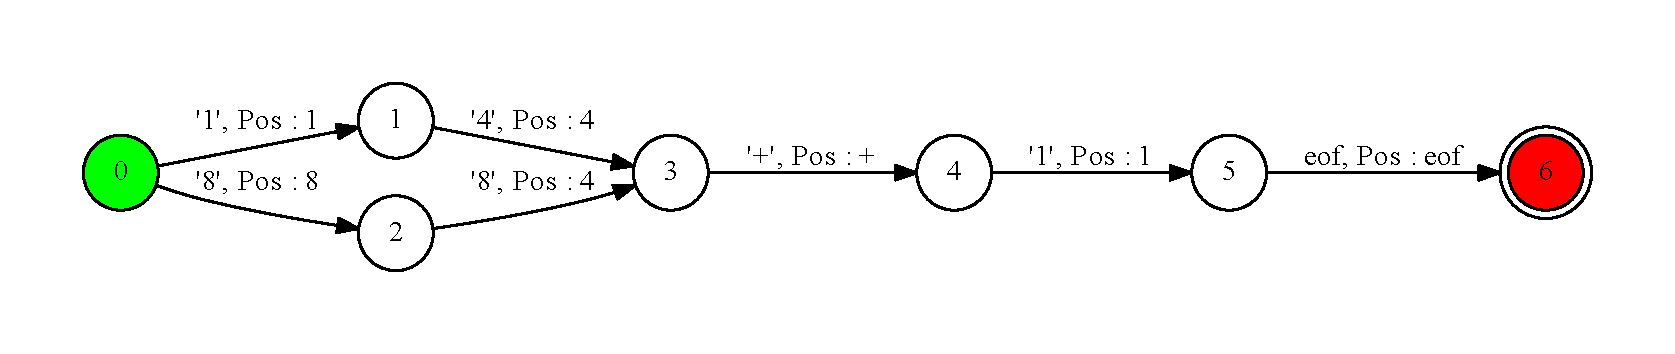
\includegraphics[width=16cm]{pictures/example.pdf}
\caption{Конечный преобразователь, участник операции композиции FST}
\label{участник_композиции}
\end{figure}

\begin{figure}[h]
\centering
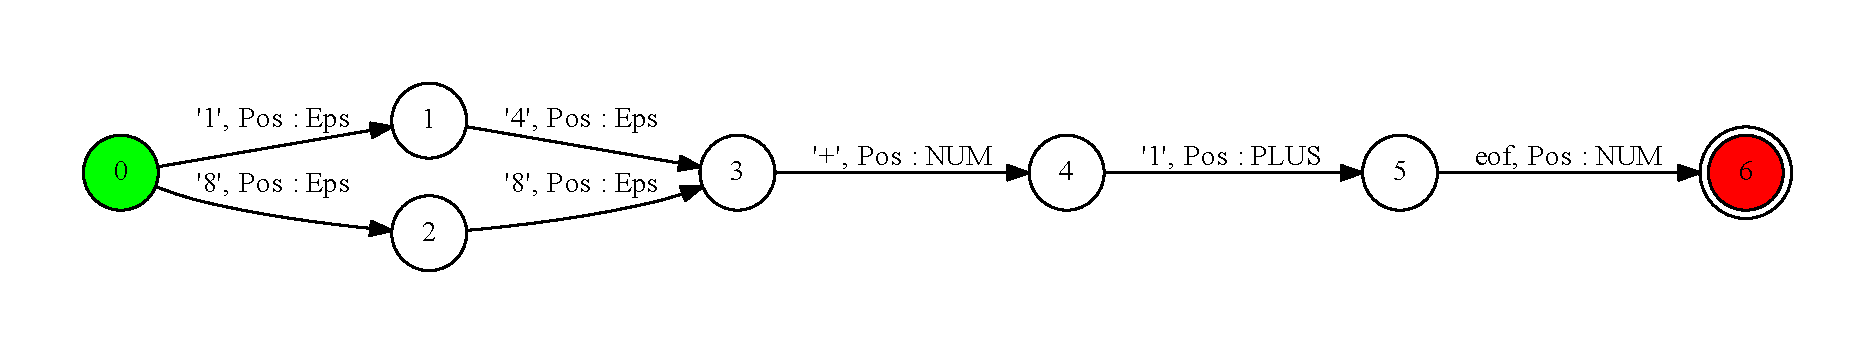
\includegraphics[width=16cm]{pictures/res.pdf}
\caption{Результат операции композиции FST}
\label{результат_композиции}
\end{figure}

В существующей реализации операция композиции является основной операцией в лексическом анализе динамически формируемых языков. Однако в проекте YaccConstructor \cite{yacc_article,yacc_www}, в рамках которого было реализовано такое решение \cite{polubelova}, ее производительность оказалась неудовлетворительной. Таким образом, целью данной работы являлось исследование возможности улучшения производительности лексического анализа за счет оптимизации алгоритма композиции конечных преобразователей.

\section{Постановка задачи}
Целью данной работы являлось исследование возможности улучшения производительности лексического анализа за счет оптимизации алгоритма композиции конечных преобразователей. Для достижения этой цели были поставлены следующие задачи.

\begin{itemize}
\item Исследовать алгоритмы композиции конечных преобразователей.
\item Реализовать и интегрировать в проект YaccConstructor более оптимальный алгоритм композиции.
\item Сравнить производительность реализаций текущего и выбранного алгоритмов.
\end{itemize} 

\section{Обзор}
Конечный преобразователь может быть задан следующей шестеркой элементов: $\langle Q, \Sigma, \Delta, q_0, F, E \rangle$, где

\begin{itemize}
\item $Q$ — множество состояний, 
\item $\Sigma$ — входной алфавит, 
\item $\Delta$ — выходной алфавит, 
\item $q_0 \in Q$ — начальное состояние, 
\item $F \subseteq Q$ — набор конечных состояний, 
\item $E \subseteq Q \times (\Sigma \cup \{\varepsilon\}) \times (\Delta \cup \{\varepsilon\})  \times Q$ — набор переходов. 
\end{itemize}

Композицией двух конечных преобразователей $T_1~=~\langle Q_1, \Sigma_1, \Delta_1, q_{0_{1}}, \\F_1, E_1 \rangle$ и $T_2~=~\langle Q_2, \Sigma_2, \Delta_2, q_{0_{2}}, F_2, E_2 \rangle$ является конечный преобразователь  $T =\langle Q_1  \times Q_2, \Sigma_1, \Delta_2, \langle q_{0_{1}}, q_{0_{2}} \rangle, F_1 \times F_2, E \cup E_{\varepsilon} \cup E_{i,\varepsilon} \cup E_{o,\varepsilon} \rangle$, где 

\begin{itemize}
\item $E = \{ \langle \langle p, q \rangle, a, b, \langle p', q' \rangle \rangle\ | \exists c \in \Delta_1 \cap \Sigma_2 : \langle p, a, c, p' \rangle \in E_1 \wedge \\\langle q, c, b, q' \rangle \in E_2\}$
\item $E_{\varepsilon} = \{ \langle \langle p, q \rangle, a, b, \langle p', q' \rangle \rangle\ | \langle p, a, {\varepsilon}, p' \rangle \in E_1 \wedge \langle q, {\varepsilon}, b, q' \rangle \in E_2\}$
\item $E_{i, \varepsilon} = \{ \langle \langle p, q \rangle, {\varepsilon}, a, \langle p, q' \rangle \rangle\ | \langle q, {\varepsilon}, a, q' \rangle \in E_2 \wedge p \in Q_1 \} $
\item $E_{o, \varepsilon} = \{ \langle \langle p, q \rangle,  a, {\varepsilon}, \langle p', q \rangle \rangle\ | \langle p, a, {\varepsilon}, p' \rangle \in E_1 \wedge q \in Q_2 \}. $
\end{itemize}

Текущая реализация алгоритма композиции FST в проекте\\ YaccConstructor работает по определению, т.е. перебирает всевозможные комбинации переходов FST участников композиции и добавляет в результирующий FST ребра, удовлетворяющие формальным описаниям из определения композиции. Поэтому временная сложность текущего алгоритма представляется как:

\[O(E_1 * E_2)\] где E — число ребер соответствующего FST.

Для удобства эту временную сложность можно представить в следующем виде:

\[O(V_1 * V_2 * D_1 * D_2)\] где V — число вершин, а D — максимальное число исходящих ребер соответствующего FST.

Важно заметить, что в результате работы алгоритма, несмотря на его корректность, в результирующем FST образуется множество недостижимых вершин, которые в дальнейшем с целью улучшения производительности, приходится удалять.

На замену текущему алгоритму был предложен алгоритм, представленный в статье \cite{handbook_automata}, потому что в результате его работы не образуется недостижимых вершин и он обладает лучшей асимптотической сложностью:

\[O(V_1 * V_2 * D_1 * (log(D_2) + M_2))\] где M — степень недетерминированности (максимальное количество исходящих из вершины ребер по одной метке).

Такая сложность достигается за счет поддержания очереди из пар вершин, в которых первая и вторая часть пары — вершины первого и второго FST соответственно. На каждой итерации алгоритма из очереди снимается одна пара вершин и перебираются комбинации ребер смежных этим вершинам. Далее, если метка выходного потока на ребре первого FST совпадает с меткой входного потока на ребре второго FST, то пара из вершин, в которые входят эти ребра, добавляется в очередь, а новое правило перехода добавляется в результирующий FST. Псевдокод алгоритма представлен в листинге (\ref{псевдокод}).

\begin{rualgorithm}[h]
 $Q\gets I_1\times I_2$\\
 $K\gets I_1\times I_2$\\
 \While{$K\neq \emptyset$}{
   $q = (q_1, q_2)\gets Head(K)$\\
   $Dequeue(K)$\\
   \If{$q \in I_1\times I_2$}{
     $I \gets I \bigcup \{q\}$\\
   }
   \If{$q \in F_1\times F_2$}{
     $F \gets F \bigcup \{q\}$\\
   }
   \For{each $(e_1, e_2) \in E[q_1] \times E[q_2]$ such that $output[e_1] = input[e_2]$}{
     $q' = (target[e_1], target[e_2])$\\
     \If{$q' \notin Q$}{
       $Q\gets Q \bigcup \{q'\}$\\
       $Enqueue(K, q')$\\
     }
     $E\gets E \bigcup \{(q, input[e_1], output[e_2], q')\}$\\
   }
 }
 \KwRet $T$\\
 \caption{Композиция FST}
 \label{псевдокод}
\end{rualgorithm}

Алгоритм возвращает новый FST $T$, множеством начальных вершин в котором является $I$, множеством конечных вершин — $F$, а множеством правил перехода — $E$. За основную очередь алгоритма обозначено $K$, а за $Q$ — множество посещенных вершин, которое помогает предотвратить зацикливание алгоритма на входах с циклами.

\section{Реализация}
\subsection{Реализация алгоритма}
Алгоритм был реализован на языке F\# семейства .NET в библиотеке для работы с конечными преобразователями YC.FST \cite{polubelova}. Можно выделить следующие особенности реализации.
\begin{itemize}
\item Класс конечных преобразователей в этой библиотеке поддерживает только целые числа в качестве состояний, но не кортежи из целых чисел, как это представляется в псевдокоде алгоритма. Поэтому было принято решение отображать сжатые представления кортежей из целых чисел в целые числа.
\item Для проверки корректности работы алгоритма были написаны модульные тесты, в которых производится композиция и сравнение FST, составленных вручную.
\end{itemize} 


\subsection{Интеграция}
В процессе работы была произведена реорганизация проекта\\ YaccConstructor, одной из целей которой являлось получение возможности сравнения производительности текущего и выбранного алгоритмов. В рамках интеграции были выполнены следующие задачи.

\begin{itemize}
\item Библиотека YC.FST была интегрирована в библиотеку для работы с графами QuickGraph \cite{quick_graph}.
\item Был произведен рефакторинг, заключавшийся в подмене сторонней библиотеки QuickGraph в YaccConstructor на использование собственной сборки этой библиотеки.
\item Библиотека для работы с позициями в тексте YC.Utils.SourceText \cite{source_text} была интегрирована в проект YaccConstructor с целью ее дальнейшего использования при оптимизации алгоритма лексического анализа.
\end{itemize} 

\section{Экспериментальное исследование}
Сравнение производительности было произведено на заранее построенных регулярных аппроксимациях, построенных по реальному коду, в котором запросы T-SQL (Transact-SQL) формируются динамически, и лексическом анализаторе T-SQL. Результаты измерений в таблице~\ref{таблица_измерений} показывают, что реализация выбранного алгоритма дает существенный прирост в производительности как на небольших синтетических примерах, так и на реальном коде, регулярные аппроксимации которого содержат большое количество ребер и вершин.

\begin{table}[h]
  \centering
    \begin{tabular}{ | p{3.8cm} | p{3.6cm} | p{3.7cm} | p{3.7cm} | }
  \hline
  Кол-во вершин в регулярной аппроксимации &
  Кол-во ребер в регулярной аппроксимации & 
  Время работы текущего алгоритма (мс) & 
  Время работы выбранного алгоритма (мс) \\ \hline
  2 & 1 & 74 & 4 \\ \hline
  8 & 34 & 133 & 7 \\ \hline
  40 & 140 & 676 & 39 \\ \hline
  215 & 895 & 4045 & 248 \\ \hline
  310 & 687 & 7184 & 394 \\ \hline
  250 & 738 & 16526 & 1133 \\ \hline
  711 & 1766 & 30285 & 2068 \\ \hline
  \end{tabular}
  \caption{Сравнение производительности алгоритмов композиции FST, построенных по регулярным аппроксимациям динамически формируемых выражений на языке T-SQL}
  \label{таблица_измерений}
\end{table}

На выборке из 600 примеров, математическое ожидание ускорения (в количестве раз) выбранного алгоритма по сравнению с текущим равно 18.7, а среднее квадратичное отклонение равно 3.23. Однако стоит заметить, что в специфике нашей задачи выбранный алгоритм должен давать константный выигрыш в производительности для определенного языка по сравнению с текущим вне зависимости от входных данных. Но задачей данной работы являлось сравнение именно реализаций алгоритмов, а они отличаются техническими оптимизациями и необходимостью производить удаление недостижимых вершин после работы текущего алгоритма, в результате чего выигрыш в производительности перестает быть константным.

\section*{Заключение}
В ходе выполнения данной работы были получены следующие результаты.

\begin{itemize}
  \item Исследованы два различных алгоритма композиции FST.
  \item Алгоритм, обладающий лучшей производительностью, реализован и интегрирован в проект YaccConstructor.
  \item Произведено сравнение производительности реализаций алгоритмов композиции FST.
  \item Результаты работы представлены на конференции «Современные технологии в теории и практике программирования». Тезисы данной работы были опубликованы в сборнике материалов конференции.
\end{itemize} 

Код, написанный в ходе выполнения данной работы, можно найти в репозитории проекта YaccConstructor \cite{yacc_git}. В указанном репозитории автор принимал участие под учетной записью baygeldin.

В дальнейшем планируется исследование структур данных и алгоритмов для работы конечными преобразователями и позициями в тексте с целью улучшения производительности алгоритма лексического анализа. Также планируется полная поддержка и интеграция с инструментом для генерации лексических анализаторов FsLex \cite{fslex}.

\setmonofont[Mapping=tex-text]{CMU Typewriter Text}
\bibliographystyle{ugost2008ls}
\bibliography{cource_work.bib}
\end{document}
